\section{Experiment}
\label{sec:experiment}

In this section, we describe experiments that empirically evaluate the proposed method and a number of 
well known baseline approaches in the three cold-start settings described in Section~\ref{sec:problem}.


\subsection{Dataset}
We make use of two publicly available playlist dataset: the 30Music~\cite{30music2015} and AotM-2011~\cite{mcfee2012hypergraph} playlist dataset.
The Million Song Dataset~\cite{msd2011} serves as an underlying dataset where all songs in playlists are intersected with,
it also provides a few song features which we will detail later.


\begin{table}[!b]
\centering
\caption{Music playlist dataset}
\label{tab:stats_pldata}
\resizebox{\linewidth}{!}{
\begin{tabular}{lrcrcc}
\toprule
Dataset   & Songs & Playlists & Users & Songs/Playlist & Playlists/User \\
\midrule
30Music   & 45,468  & 17,457  & 8,070   & 16.3 & 2.2 \\
AotM-2011 & 114,428 & 84,710  & 14,182  & 10.1 & 6.0 \\
\bottomrule
\end{tabular}
}
\end{table}

\begin{figure*}[!t]
    \centering
    \begin{minipage}{.5\textwidth}
        \centering
        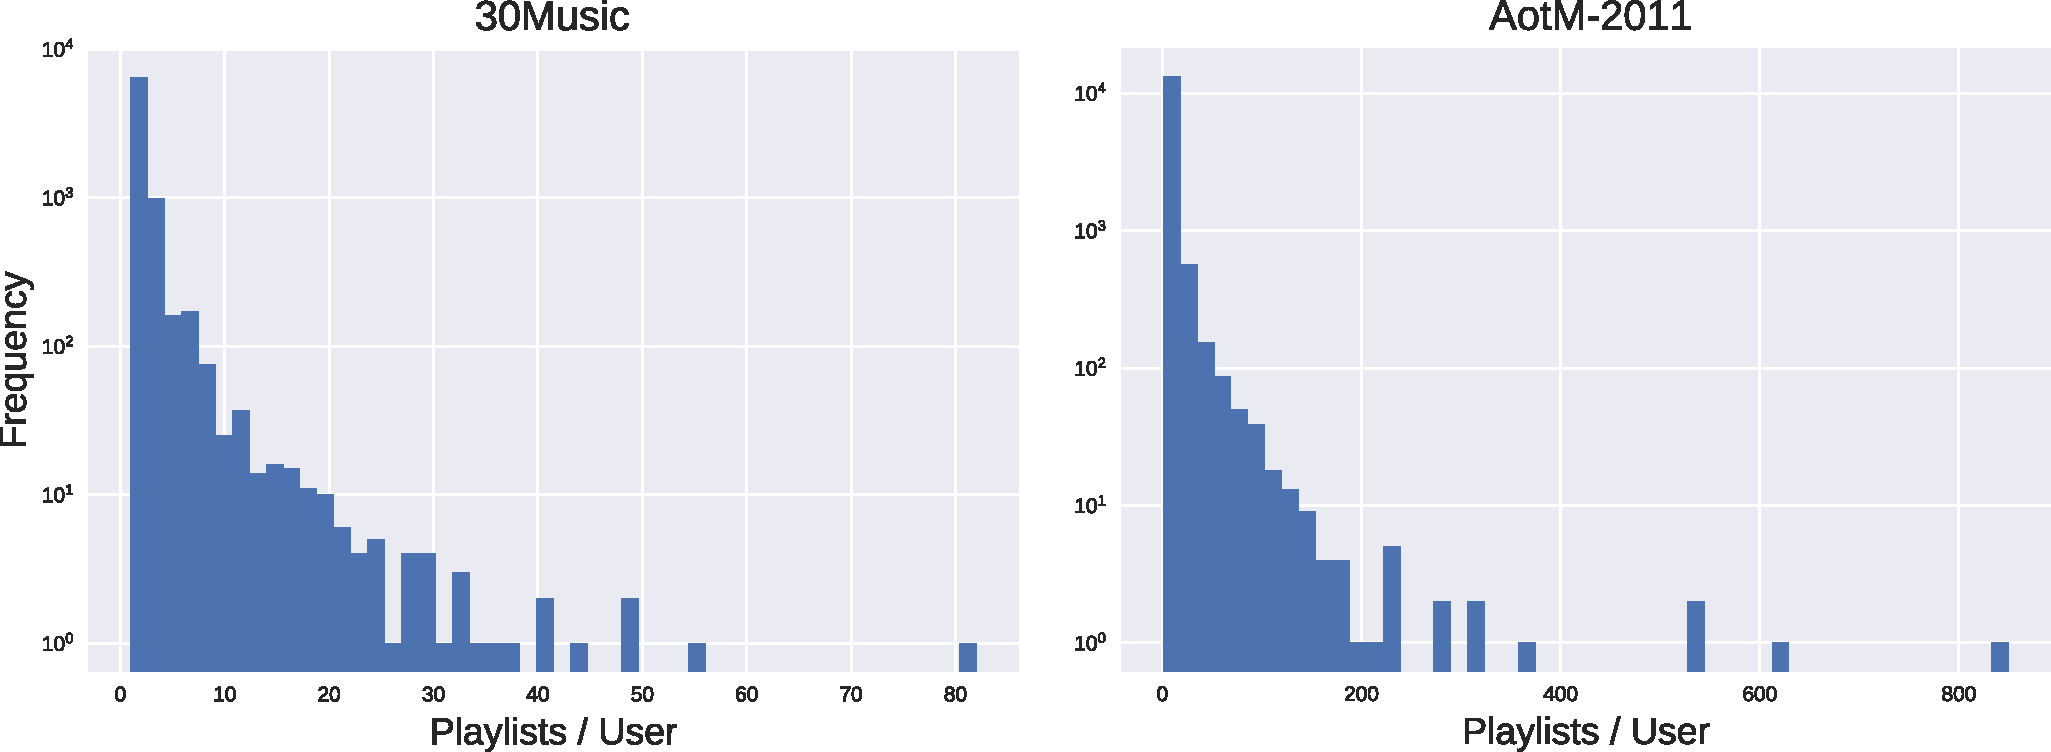
\includegraphics[width=.95\linewidth]{fig/hist_pluser.pdf}
        \caption{Histogram of the number of playlists per user}
        \label{fig:hist_pluser}
    \end{minipage}%
    \begin{minipage}{0.5\textwidth}
        \centering
        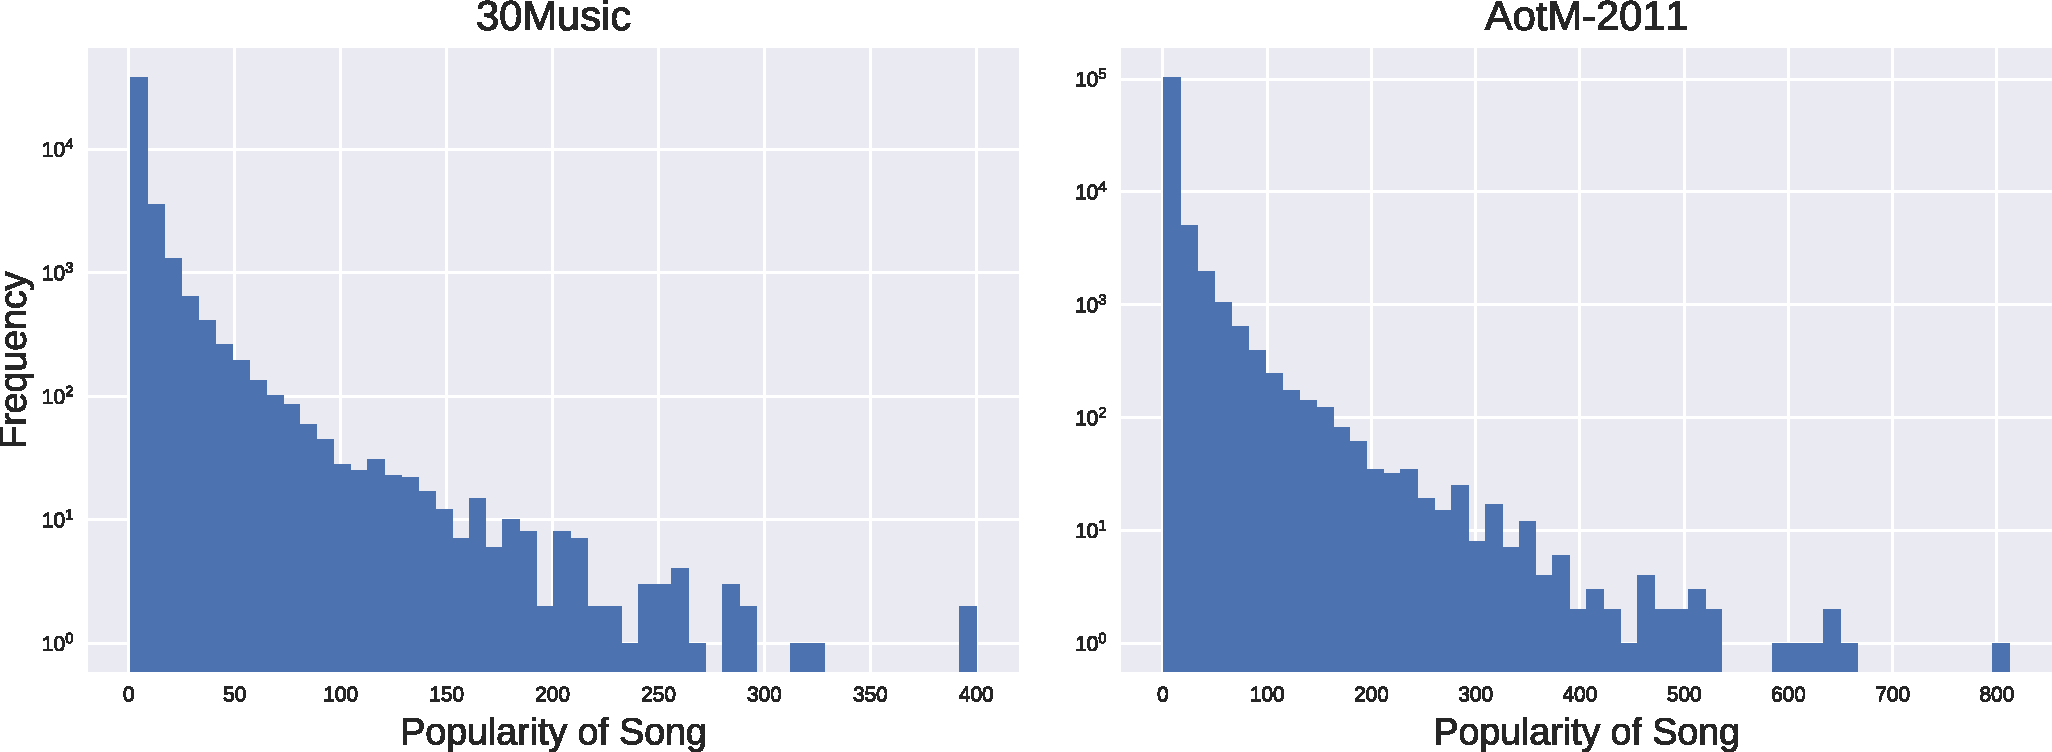
\includegraphics[width=.95\linewidth]{fig/hist_songpop.pdf}
        \caption{Histogram of song popularity}
        \label{fig:hist_songpop}
    \end{minipage}
\end{figure*}

{\bf Million Song Dataset} (MSD) is a collection of one million songs, information of each song such as the name, artist, year of release are available.
It also provides acoustic features computed from a sample section of audio file of each song. % more description

{\bf 30Music Dataset} is a collection of listening events and playlists retrieved from Last.fm\footnote{\url{https://www.last.fm}}.
We utilise the playlists data by first intersecting with the MSD, leveraging the Last.fm dataset~\cite{lastfmdataset}
which matched songs from Last.fm with those in MSD, then filtering out playlists with less than 5 songs,
which results in roughly 17K playlists over 45K songs from 8K users.

{\bf AotM-2011 Dataset} is a collection of playlists shared by users\footnote{\url{http://www.artofthemix.org}} ranging from 1998 to 2011,
songs in the dataset had been matched to those in the Million Song Dataset (MSD).
We filtered out playlists with less than 5 songs, which results in roughly 84K playlists over 114K songs from 14K users.

Table~\ref{tab:stats_pldata} summarises the two playlist dataset used in this work.
The histograms of the number of playlists per user as well as song popularity 
(\ie we use the number of occurrences of a song in all playlists as a proxy of its popularity)
of the two dataset are shown in Figure~\ref{fig:hist_pluser} and Figure~\ref{fig:hist_songpop},
respectively.
We can see from Figure~\ref{fig:hist_pluser} and \ref{fig:hist_songpop} that both the number
of playlists per user and song popularity follow a long-tail distribution, which impose further challenge to the learning task as the amount
of data for learning is limited for users (or songs) at the tail.


\begin{table*}[!t]
    \centering
    \begin{minipage}{.35\textwidth}
        \centering
        \caption{Dataset for \emph{cold songs}}
        \label{tab:stats0}
        \resizebox{.9\textwidth}{!}{
        \begin{tabular}{lrrcrr}
        \toprule
        \multirow{2}{*}{Dataset}  & \multicolumn{2}{c}{Songs} && \multicolumn{2}{c}{Playlists} \\ \cmidrule{2-3} \cmidrule{5-6}
                                  & Train & Test && Train & Test \\
        \midrule
        30Music   & 40,468  & 5,000  && 17,342  & 8,215 \\
        AotM-2011 & 104,428 & 10,000 && 84,646  & 19,504 \\
        \bottomrule
        \end{tabular}
        }
    \end{minipage}%
    \begin{minipage}{0.33\textwidth}
        \centering
        \caption{Dataset for \emph{cold playlists}}
        \label{tab:stats1}
        \resizebox{.9\textwidth}{!}{
        \begin{tabular}{lrrcrr}
        \toprule
        \multirow{2}{*}{Dataset}  & \multicolumn{2}{c}{Playlists} && \multicolumn{2}{c}{Users} \\ \cmidrule{2-3} \cmidrule{5-6}
                                  & Train & Test && Train & Test \\
        \midrule
        30Music   & 15,262 & 2,195 &&  8,070 & 1,644 \\
        AotM-2011 & 75,477 & 9,233 && 14,182 & 2,722 \\
        \bottomrule
        \end{tabular}
        }
    \end{minipage}%
    \begin{minipage}{.33\textwidth}
        \centering
        \caption{Dataset for \emph{cold users}}
        \label{tab:stats2}
        \resizebox{.9\textwidth}{!}{
        \begin{tabular}{lrrcrr}
        \toprule
        \multirow{2}{*}{Dataset}  & \multicolumn{2}{c}{Playlists} && \multicolumn{2}{c}{Users} \\ \cmidrule{2-3} \cmidrule{5-6}
                                  & Train & Test && Train & Test \\
        \midrule
        30Music   & 14,067 & 3,390 && 5,649 & 2,421 \\
        AotM-2011 & 76,450 & 8,260 && 9,928 & 4,254 \\
        \bottomrule
        \end{tabular}
        }
    \end{minipage}
\end{table*}




\subsection{Experimental setup}

We describe how playlist data are split into training and test set for all three cold-start settings,
features of songs used to learn the multitask objective, as well as baseline approaches and evaluation metrics.

{\bf Dataset split}.
To empirically evaluate the performance of recommending new songs to extend existing playlists (setting (i)),
we hold 5K of the latest released songs in 30Music dataset, which results in about 8K playlists with songs
in both training and test set.
We hold 10K of the latest released songs in AotM-2011 dataset, which leads to about 19K playlists with songs
in both training and test set.
Playlists that all songs have been held are removed from both training and test set.
Table~\ref{tab:stats0} summarises the statistics of this training/test split.

For the task of recommending songs to form playlists for existing users (setting (ii)),
%To empirically evaluate the performance of our proposed recommendation approaches for existing users,
we hold playlists from about 20\% users in both datasets for test, all other playlists are used for training.
To make sure each song in test set also appeared in training set,
and all users in test set also have a few playlists in training set.
The test set are sampled from users that have at least one playlist where each song has also been
included in four other playlists among the whole dataset,
which results in a test set with about 2.1K playlists from 1.6K users in 30Music dataset,
and a test set with about 9.2K playlists from 2.7K users in AotM-2011 dataset.
The statistics of this training/test split are shown in Table~\ref{tab:stats1}.

To evaluate the last cold-start setting (iii), \ie recommending songs to form playlist for new users,
%To evaluate the performance of music recommendation approaches for new users,
we sampled 30\% of all users and hold all their playlists as test set in both datasets.
Similarly, to make sure songs in test set also exist in training set,
a user is not sampled when holding all of her playlists breaks this requirement.
This results in a test set with about 3.4K playlists from 2.4K users in 30Music dataset,
and a test set with about 8.2K playlists from 4.2K users in AotM-2011 dataset.
Table~\ref{tab:stats2} describes the statistics of this training/test split.


{\bf Features}.
Song features used in experiment including metadata, audio data, genre and artist information, and song/artist popularity.
%
The metadata of songs (\eg duration, year of release) and audio features (\eg loudness, mode, tempo) are provided by MSD.
We use genre data from the Top-MAGD genre dataset~\cite{schindler2012facilitating}
and tagtraum genre annotations for MSD~\cite{schreiber2015improving} via one-hot encoding.
If the genre data of a song is not available, we apply the mean imputation using genre counts of other songs in training set.
To encode artist information as features,
we trained a word2vec\footnote{https://github.com/dav/word2vec} model using sequences of artist names in playlists.

In the task of recommending new songs to extend existing playlists (setting (i)), where song popularity is not available,
we use artist popularity (we use the number of occurrences of all songs from a artist in training playlists as a proxy of her popularity).
Finally, we add a constant feature (with value $1$) for each song to account for bias.


{\bf Baselines}.
We compare the performance of our proposed approach (referred as {\it Multitask Classification}) 
with a number of baseline methods for the task of recommending music to form playlists:
\begin{itemize}
\item The {\it Popularity Ranking} method scores each song using only its popularity in training set, 
      when song popularity is not available (setting (i)), we use artist popularity.
\item The {\it Same Artists - Greatest Hits} (SAGH)~\cite{mcfee2012million} method scores scores each song
      by its popularity if the artist of the song has appeared in the given user's playlist in training set,
      otherwise the song is scored zero.
      Similarly, we replace song popularity with artist popularity in the task of recommending new songs (setting (i)).
\item The {\it Collocated Artists - Greatest Hits} (CAGH)~\cite{bonnin2013evaluating} method is a variant of SAGH.
      It scores each song using its popularity, but weighted by the frequency of the collocation between artist of the song
      and those artists that appeared in the given user's playlist in training set.
      In the task of recommending new songs (setting (i)), we again replace the song popularity in this method with artist popularity.
      When recommending songs for new users (setting (iii)), we use the top 10 most popular artists instead of artists in the user's
      listening history as required by this method.
\item The {\it Logistic Regression} baseline is specific for the task of recommending new songs (setting (i)), where we independenly train
      an logistic regression classifier for each playlist, which is used to classify each new song whether we should add it to this playlist.
      This method is also known as binary relevance in multi-label classification.
\end{itemize}


{\bf Evaluation}.
We evaluate the performance of all approaches using two metrics that are commonly employed in playlist recommendation tasks:
Hit-Rate@K~\cite{hariri2012context} and Area under the ROC curve (AUC)~\cite{manning2008introIR}.
%
%R-Precision (RPREC) is the number of correctly recommended songs in the top-$n$ recommendation over $n$,
%where $n$ is the number of songs in the ground truth playlist.
%It is one of several metrics used to evaluate performance on playlist continuation tasks
%in the ACM RecSys Challenge 2018\footnote{https://recsys-challenge.spotify.com/rules}.
%
Hit-Rate@K (or Hit Ratio) is the number of correctly recommended songs among top-$K$ recommendation over $L$,
where $K$ is the number of recommendations, and $L$ is the number of songs in the ground truth playlist.
It has been employed to evaluate several playlist generation and next song recommendation
methods~\cite{hariri2012context,bonnin2013evaluating,bonnin2015automated,jannach2015beyond}.
This metric is also known as Recall@K~\cite{schedl2017}.
%
The area under the ROC curve (AUC) is widely used in measuring performance of classifiers,
it has also been used for evaluating performance of playlist generation method when the task
is cast as a (sequence of) classification problem~\cite{ben2017groove}.


\subsection{Results and discussion}

We can see from Table~\ref{tab:perf0} that learning based methods (\ie {\bf Multitask classification}
and {\it Logistic Regression} perform significantly better than other baselines, in the setting of
recommending new songs for extending playlists (setting (i)).
Which suggests learning from existing playlists helps the task of recommending new songs.
Among the (artist) popularity based approaches, 
simply ranking songs by its artist popularity achieves decent performance,
and take into account artist collocation information does not seem to improve the performance.
Further, the SAGH method which considers only songs from the top 10 most popular artists,
is the worst performer in terms of HitRate@100 and AUC.

Figure~\ref{fig:hr0} shows the hit rates when the number of recommendations $K$ varies from 0 to 1000.
We can see that the performance of all methods improves as the number of recommendations increase,
and learning based methods are always performing better than ranking based artist informations.
It is interesting that both {\it Multitask Classification} and {\it Logistic Regression} perform 
almost the same when $K$ is small (100 on 30Music and 50 on AotM-2011 dataset), 
and the former only performance better when $K$ is big than that.
Another interesting observation is that SAGH and CAGH performs similar on AotM-2011 dataset when $K$
is less 50, and both outperforms {\it Popularity Ranking}, however, SAGH suffer from slow improvement
as $K$ increases, this effect is observed on both datasets.


\begin{table}[h]
\centering
\caption{Performance in setting (i)}
\label{tab:perf0}
\resizebox{\columnwidth}{!}{
\begin{tabular}{l*{4}{c}*{4}{c}}
\toprule
\multirow{2}{*}{Method}      & \multicolumn{2}{c}{30Music} && \multicolumn{2}{c}{AotM-2011} \\ \cmidrule{2-3} \cmidrule{5-6}
                             & HitRate@100 \% & AUC \% && HitRate@100 \% & AUC \% \\
\midrule
SAGH &                   \hspace{0.45em}$4.8$ & $51.6$ && \hspace{0.2em} $7.8$ & $53.6$ \\
CAGH &                                 $10.9$ & $69.2$ &&               $11.9$ & $77.5$ \\
Popularity Ranking &                   $12.2$ & $70.9$ && \hspace{0.2em} $8.7$ & $76.5$ \\
Logistic Regression &                  $35.4$ & $82.5$ &&               $23.1$ & $81.0$ \\
Multitask Classification & ${\bf 36.2}$ & ${\bf 86.6}$ &&         ${\bf 24.4}$ & ${\bf 84.3}$ \\
\bottomrule
\end{tabular}

}
\end{table}

\begin{figure}[h]
\centering
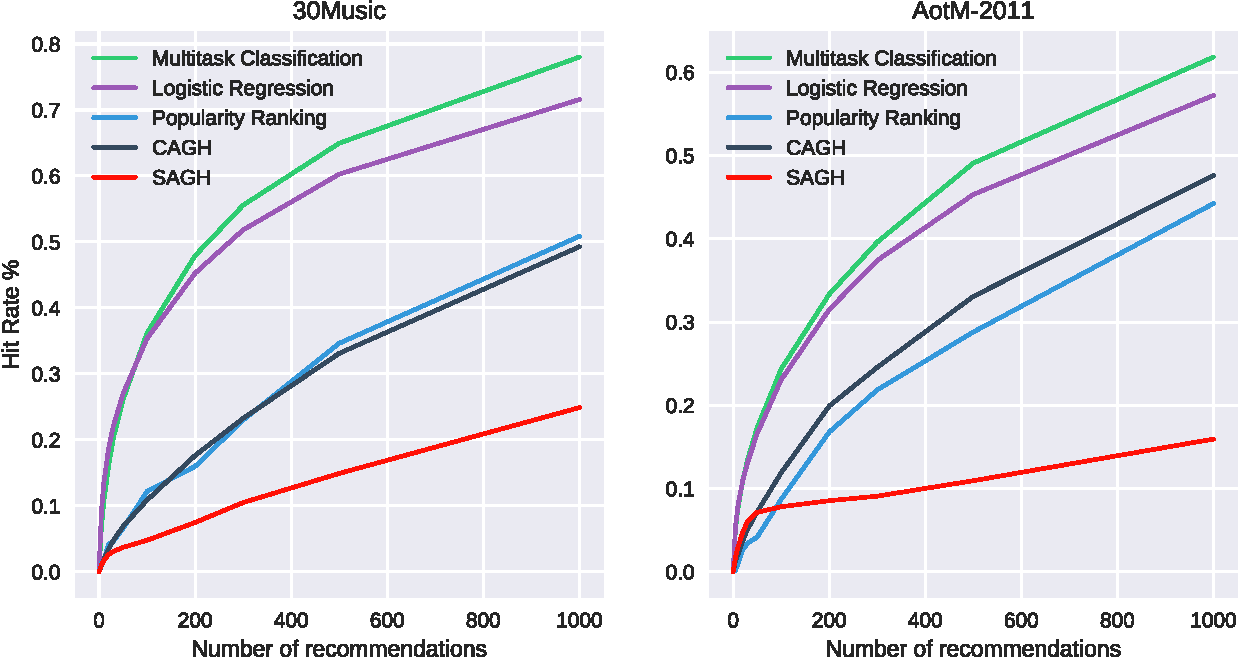
\includegraphics[width=.975\linewidth]{fig/hitrate0.pdf}
\caption{Hit rates in setting (i)}
\label{fig:hr0}
\end{figure}


Table~\ref{tab:perf1} and Figure~\ref{fig:hr1} show the performance on the task of recommending a set of songs for
an existing user (setting (ii)).
First, we can see that methods based on song popularity and artist information achieve good performance,
which is in line with discoveries in~\cite{bonnin2013evaluating,jannach2015beyond,bonnin2015automated} which 
show ranking based on popularity is a strong baseline.
Further, methods which make use of both song popularity and artist information,
outperform {\it Popularity Ranking} (except SAGH on 30Music), which shows artist information is helpful for music recommendation,
which is consistent with results reported in~\cite{bonnin2013evaluating,bonnin2015automated}.
%
%It is interesting to see that {\it Popularity Ranking}) perform worse than other methods in terms of HitRate@100,
%but SAGH performs worse than other methods in terms of AUC,
%which might suggest that SAGH achieves good recall but {\it Popularity Ranking} performs better on average.
It is interesting to observe that SAGH is one of the best performer on AotM-2011 dataset (Figure~\ref{fig:hr1}), 
while it performs the worst in terms of HitRate@K on 30Music dataset, when $K$ is greater than 300.
%The performance of SAGH is also saturated much earlier than other methods.
%
%performance of all methods improves when $K$ increases, and {\it Multitask Classification}
%achieves the best performance on both datasets.
%However, while CAGH performs as good as {\it Multitask Classification} on 30Music,
%it is SAGH that achieves the best performance among all methods that ranks song by popularity and artist information
%on the AotM-2011 dataset, this might reflect the different characteristics between the two playlist dataset.


\begin{table*}[!t]
    \centering
    \begin{minipage}{.5\textwidth}
        \centering
        \caption{Performance in setting (ii)}
        \label{tab:perf1}
        \resizebox{.95\textwidth}{!}{
        \begin{tabular}{l*{4}{c}*{4}{c}}
\toprule
\multirow{2}{*}{Method}      & \multicolumn{2}{c}{30Music} && \multicolumn{2}{c}{AotM-2011} \\ \cmidrule{2-3} \cmidrule{5-6}
                             & HitRate@100 \% & AUC \% && HitRate@100 \% & AUC \% \\
\midrule
SAGH &                   \hspace{0.45em}$4.8$ & $51.6$ && \hspace{0.2em} $7.8$ & $53.6$ \\
CAGH &                                 $10.9$ & $69.2$ &&               $11.9$ & $77.5$ \\
Popularity Ranking &                   $12.2$ & $70.9$ && \hspace{0.2em} $8.7$ & $76.5$ \\
Logistic Regression &                  $35.4$ & $82.5$ &&               $23.1$ & $81.0$ \\
Multitask Classification & ${\bf 36.2}$ & ${\bf 86.6}$ &&         ${\bf 24.4}$ & ${\bf 84.3}$ \\
\bottomrule
\end{tabular}

        }
    \end{minipage}%
    \begin{minipage}{0.5\textwidth}
        \centering
        \caption{Performance in setting (iii)}
        \label{tab:perf2}
        \resizebox{.95\textwidth}{!}{
        %\begin{table}[!h]
%\centering
%\caption{Performance of recommendation for new users}
%\label{tab:perf_plgen2}
%\resizebox{\columnwidth}{!}{
\begin{tabular}{l*{4}{c}*{4}{c}}
\toprule
\multirow{2}{*}{Method}  & \multicolumn{2}{c}{30Music} && \multicolumn{2}{c}{AotM-2011} \\ \cmidrule{2-3} \cmidrule{5-6}
                         & RPREC \textperthousand & AUC \% && RPREC \textperthousand & AUC \% \\
\midrule
Popularity Rank &           $21.4$ & $88.3$ &&                       $13.5$ & $91.8$ \\
Top10 SAGH &                $19.6$ & $54.5$ &&                       $11.5$ & $53.7$ \\
Top10 CAGH &                $19.5$ & $87.3$ &&                       $11.5$ & $89.4$ \\
Multitask Classification &  $21.0$ & $88.8$ &&                       $13.5$ & $91.6$ \\
Multitask Ranking &            N/A &    N/A &&                          N/A &    N/A \\
\bottomrule
\end{tabular}
%}
%\end{table}

        }
    \end{minipage}
\end{table*}


\begin{figure*}[t]
    \centering
    \begin{minipage}{.5\textwidth}
        \centering
        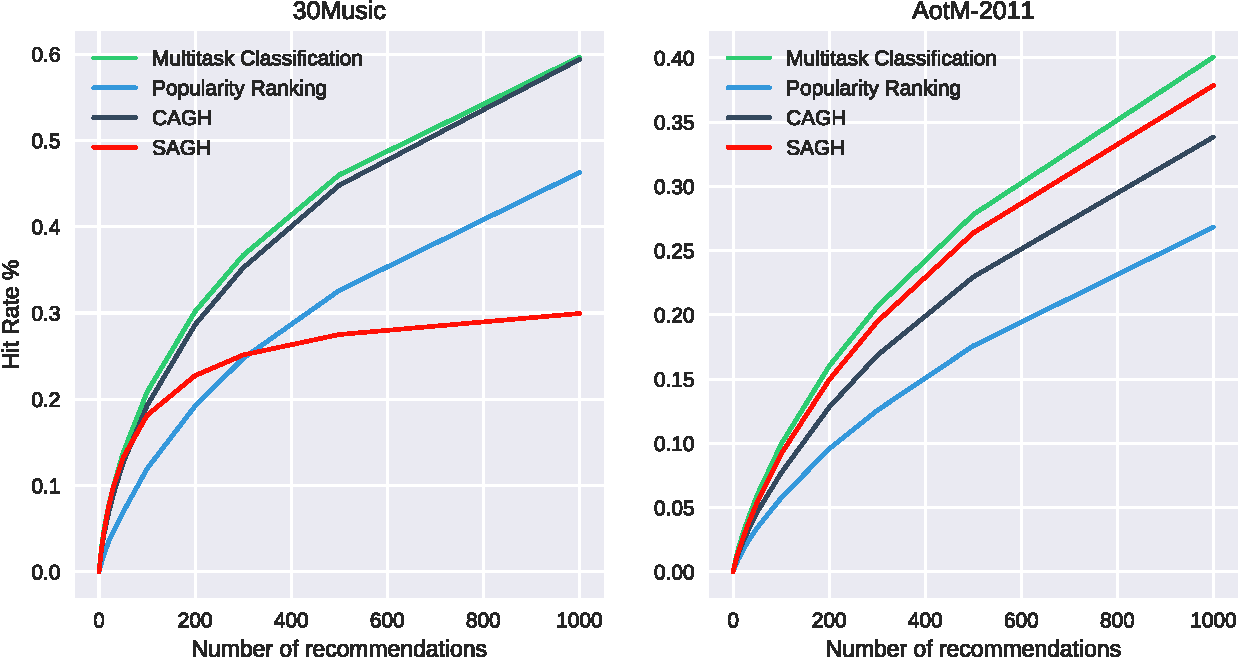
\includegraphics[width=.925\linewidth]{fig/hitrate1.pdf}
        \caption{Hit rates in setting (ii)}
        \label{fig:hr1}
    \end{minipage}%
    \begin{minipage}{0.5\textwidth}
        \centering
        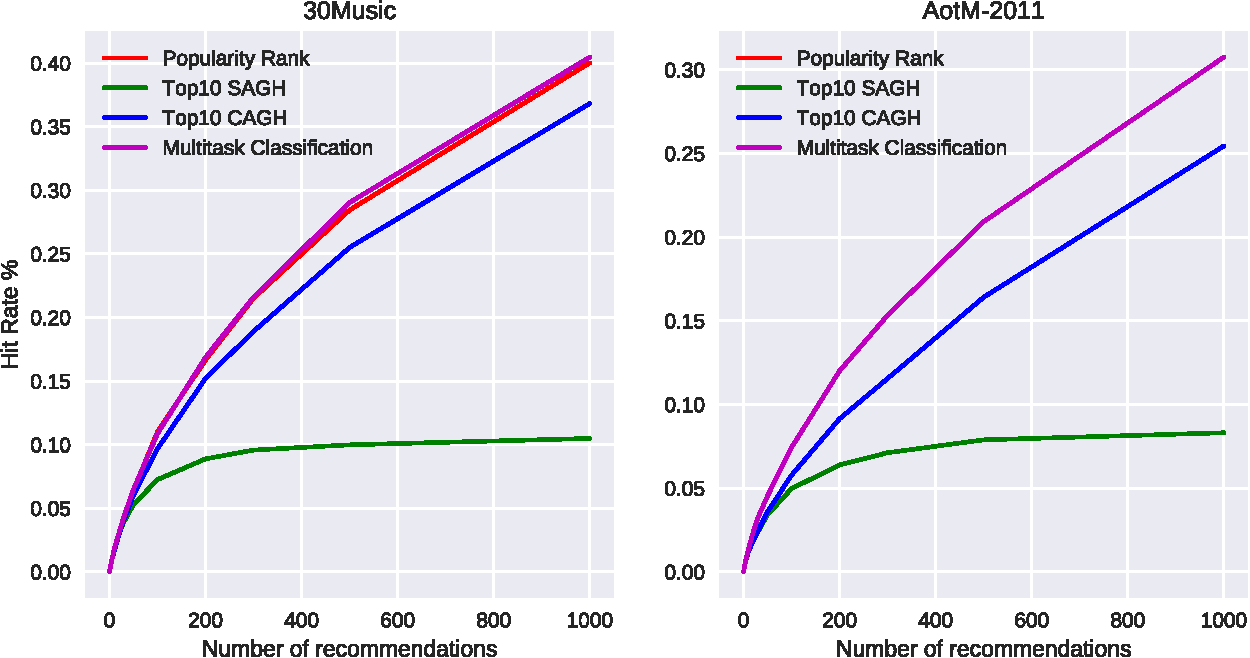
\includegraphics[width=.925\linewidth]{fig/hitrate2.pdf}
        \caption{Hit rates in setting (iii)}
        \label{fig:hr2}
    \end{minipage}
\end{figure*}



Finally, the performance in the setting of recommending music to form playlists for new users (setting (iii)),
however, is quite different from the other two cold-start settings.
%
We can see from Table~\ref{tab:perf2} and Figure~\ref{fig:hr2} that {\it Popularity Ranking} is one of the best performing methods,
outperforming both baselines that make use of song popularity and artist information (\ie SAGH and CAGH).
The performance of {\it Multitask Classification} is almost identical to that of {\it Popularity Ranking} in terms of all metrics,
which suggests {\it Multitask Classification} might degenerate to simply rank songs using its popularity.
Another interesting observation is that, although both SAGH and CAGH make use of song popularity and artist information,
the later performs significantly better than the former in terms of AUC and HitRate@K (when $K$ is greater than 100).
This suggests the way to make use of artist information matters,
and collocation of artists could be more helpful for music recommendation than simply filtering out songs 
that are not from popular artists.

Last but not the least, our proposed method {\it Multitask Classification}, unlike any other method in consideration,
has always been one of the best performer in all three cold-start settings on both datasets,
Which suggests our propose approach can work effectively for the cold-start settings considered in this paper.
As a remark, the performance of all methods in terms of HitRate@K improve as the number of recommendations increase,
and the rate of improvement decreases as more songs are recommended.
In particular, the performance of SAGH tends to saturate much earlier than other methods (except in setting (ii) on AotM-2011 dataset),
which might suggest that, as more songs are recommended, artists in users' listening history (or popular artists) become less informative,
and other factors such as song popularity regains its dominance for the task of music recommendation.



